% =========================================================================
% KHO TÀI NGUYÊN MẪU TIKZ CHÍNH THỨC - DỰ ÁN LA-TEX-TO-PIC
% Hệ thống Base Models (Cấu trúc Topology Gốc)
% =========================================================================
\documentclass[12pt,a4paper,oneside]{book}
\usepackage{fouriernc}
\usepackage{amsmath,amssymb}
\usepackage{tikz,tkz-tab,tkz-euclide,pgfplots}
\pgfplotsset{compat=1.15}
\usepackage[top=1.5cm, bottom=1.5cm, left=1.2cm, right=1.2cm] {geometry}
\usepackage[dethi]{ex_test}

% Khai báo thư viện tcolorbox để kẻ khung mã source code
\usepackage[many,most]{tcolorbox}
\tcbuselibrary{listings}

% Style chuẩn cho tcolorbox mã nguồn
\tcbset{
  codebox/.style={
    colback=gray!5,
    colframe=blue!60!black,
    boxrule=1pt,
    arc=3pt,
    title=Code TikZ Base,
    left=2mm, right=2mm, top=1mm, bottom=1mm,
    fontupper=\scriptsize\ttfamily
  }
}

\begin{document}
\Opensolutionfile{ans}

\begin{center}
    \LARGE \textbf{BỘ KHUNG MẪU HÌNH VẼ TIKZ CHÍNH THỨC (BASE TOPOLOGY)}
    
    \Large \textit{Phục vụ render động trên Streamlit Web App}
\end{center}

\vspace{1cm}

% -------------------------------------------------------------------------
\section*{A. NHÓM CHÓP TAM GIÁC SERIES}
% -------------------------------------------------------------------------

\subsection*{A.1. Chóp tam giác - Cạnh bên vuông góc đáy (SA $\perp$ ABC)}
\noindent
\begin{minipage}[c]{0.45\textwidth}
\centering
\begin{tikzpicture}[scale=1,>=stealth, font=\footnotesize, line join=round, line cap=round]
	\tkzDefPoints{0/0/A,1.2/-1.5/B,4/0/C}
	\coordinate (S) at ($(A)+(0,3)$);
	\tkzDrawPolygon(S,A,B,C)
	\tkzDrawSegments(S,B)
	\tkzDrawSegments[dashed](A,C)
	\tkzDrawPoints[fill=black,size=4](A,B,C,S)
	\tkzMarkRightAngles[size=0.16](S,A,B S,A,C)
	\tkzLabelPoints[above](S)
	\tkzLabelPoints[below](B)
	\tkzLabelPoints[left](A)
	\tkzLabelPoints[right](C)
\end{tikzpicture}
\end{minipage}\hfill
\begin{minipage}[c]{0.52\textwidth}
\begin{tcolorbox}[codebox]
\begin{verbatim}
\begin{tikzpicture}[scale=1,>=stealth,
    font=\footnotesize, line join=round, line cap=round]
  \tkzDefPoints{0/0/A,1.2/-1.5/B,4/0/C}
  \coordinate (S) at ($(A)+(0,3)$);
  \tkzDrawPolygon(S,A,B,C)
  \tkzDrawSegments(S,B)
  \tkzDrawSegments[dashed](A,C)
  \tkzDrawPoints[fill=black,size=4](A,B,C,S)
  \tkzMarkRightAngles[size=0.16](S,A,B S,A,C)
  \tkzLabelPoints[above](S)
  \tkzLabelPoints[below](B)
  \tkzLabelPoints[left](A)
  \tkzLabelPoints[right](C)
\end{tikzpicture}
\end{verbatim}
\end{tcolorbox}
\end{minipage}

\vspace{0.5cm}

\subsection*{A.2. Chóp tam giác - Mặt bên vuông góc đáy (SAB $\perp$ ABC)}
\noindent
\begin{minipage}[c]{0.45\textwidth}
\centering
\begin{tikzpicture}[scale=1,>=stealth, font=\footnotesize, line join=round, line cap=round]
	\tkzDefPoints{0/0/A,1.2/-1.8/B,4.5/0/C}
	\coordinate (H) at ($(A)!0.5!(B)$); % H là trung điểm AB
	\coordinate (S) at ($(H)+(0,3)$);    % SH vuông góc ABC
	\tkzDrawPolygon(S,A,B,C)
	\tkzDrawSegments(S,B)
	\tkzDrawSegments[dashed](A,C S,H)
	\tkzDrawPoints[fill=black,size=4](A,B,C,S,H)
	\tkzMarkRightAngles[size=0.16](S,H,A S,H,C)
	\tkzLabelPoints[above](S)
	\tkzLabelPoints[below](B)
	\tkzLabelPoints[left](A)
	\tkzLabelPoints[right](C)
	\tkzLabelPoints[below left](H)
\end{tikzpicture}
\end{minipage}\hfill
\begin{minipage}[c]{0.52\textwidth}
\begin{tcolorbox}[codebox]
\begin{verbatim}
\begin{tikzpicture}[scale=1,>=stealth,...]
  \tkzDefPoints{0/0/A,1.2/-1.8/B,4.5/0/C}
  \coordinate (H) at ($(A)!0.5!(B)$); 
  \coordinate (S) at ($(H)+(0,3)$);    
  \tkzDrawPolygon(S,A,B,C)
  \tkzDrawSegments(S,B)
  \tkzDrawSegments[dashed](A,C S,H)
  \tkzDrawPoints[fill=black,size=4](A,B,C,S,H)
  \tkzMarkRightAngles[size=0.16](S,H,A S,H,C)
  \tkzLabelPoints[above](S)
  \tkzLabelPoints[left](A) ...
\end{tikzpicture}
\end{verbatim}
\end{tcolorbox}
\end{minipage}

\vspace{1cm}

% -------------------------------------------------------------------------
\section*{B. NHÓM CHÓP TỨ GIÁC SERIES}
% -------------------------------------------------------------------------

\subsection*{B.1. Chóp tứ giác đáy HBH - Cạnh bên vuông góc đáy (SA $\perp$ ABCD)}
\noindent
\begin{minipage}[c]{0.45\textwidth}
\centering
\begin{tikzpicture}[scale=0.9,>=stealth, font=\footnotesize, line join=round, line cap=round]
	\tkzDefPoints{0/0/A, -1.5/-1.5/B, 3/-1.5/C}
	\coordinate (D) at ($(A)+(C)-(B)$);
	\coordinate (S) at ($(A)+(0,3)$);
	\tkzDrawPolygon(S,B,C,D)
	\tkzDrawSegments(S,C)
	\tkzDrawSegments[dashed](S,A A,B A,D)
	\tkzDrawPoints[fill=black,size=4](A,B,C,D,S)
	\tkzMarkRightAngles[size=0.16](S,A,B S,A,D)
	\tkzLabelPoints[above](S)
	\tkzLabelPoints[below](B,C)
	\tkzLabelPoints[left](A)
	\tkzLabelPoints[right](D)
\end{tikzpicture}
\end{minipage}\hfill
\begin{minipage}[c]{0.52\textwidth}
\begin{tcolorbox}[codebox]
\begin{verbatim}
\begin{tikzpicture}[scale=0.9,>=stealth,...]
  \tkzDefPoints{0/0/A, -1.5/-1.5/B, 3/-1.5/C}
  \coordinate (D) at ($(A)+(C)-(B)$);
  \coordinate (S) at ($(A)+(0,3)$);
  \tkzDrawPolygon(S,B,C,D)
  \tkzDrawSegments(S,C)
  \tkzDrawSegments[dashed](S,A A,B A,D)
  \tkzDrawPoints[fill=black,size=4](A,B,C,D,S)
  \tkzMarkRightAngles[size=0.16](S,A,B S,A,D)
  \tkzLabelPoints[above](S) ...
\end{tikzpicture}
\end{verbatim}
\end{tcolorbox}
\end{minipage}

\vspace{0.5cm}

\subsection*{B.2. Chóp tứ giác đều (SO $\perp$ ABCD)}
\noindent
\begin{minipage}[c]{0.45\textwidth}
\centering
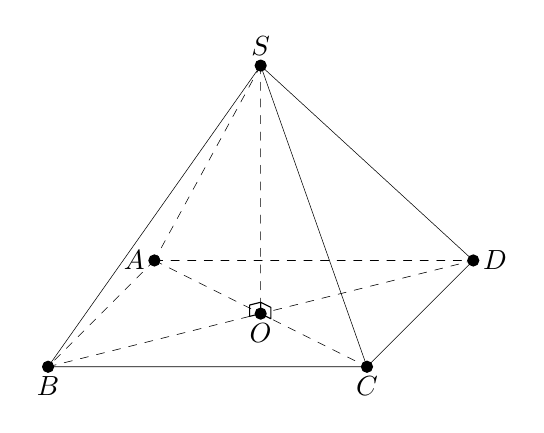
\begin{tikzpicture}[scale=0.9,>=stealth, font=\footnotesize, line join=round, line cap=round]
	\tkzDefPoints{0/0/A, -1.5/-1.5/B, 3/-1.5/C}
	\coordinate (D) at ($(A)+(C)-(B)$);
	\coordinate (O) at ($(A)!0.5!(C)$);
	\coordinate (S) at ($(O)+(0,3.5)$);
	\tkzDrawPolygon(S,B,C,D)
	\tkzDrawSegments(S,C)
	\tkzDrawSegments[dashed](S,A A,B A,D A,C B,D S,O)
	\tkzDrawPoints[fill=black,size=4](A,B,C,D,S,O)
	\tkzMarkRightAngles[size=0.16](S,O,B S,O,C)
	\tkzLabelPoints[above](S)
	\tkzLabelPoints[below](B,C,O)
	\tkzLabelPoints[left](A)
	\tkzLabelPoints[right](D)
\end{tikzpicture}
\end{minipage}\hfill
\begin{minipage}[c]{0.52\textwidth}
\begin{tcolorbox}[codebox]
\begin{verbatim}
\begin{tikzpicture}[scale=0.9,>=stealth,...]
  \tkzDefPoints{0/0/A, -1.5/-1.5/B, 3/-1.5/C}
  \coordinate (D) at ($(A)+(C)-(B)$);
  \coordinate (O) at ($(A)!0.5!(C)$);
  \coordinate (S) at ($(O)+(0,3.5)$);
  \tkzDrawPolygon(S,B,C,D)
  \tkzDrawSegments(S,C)
  \tkzDrawSegments[dashed](S,A A,B A,D 
                           A,C B,D S,O)
  \tkzDrawPoints[fill=black,size=4](A,B,C,D,S,O)
  \tkzMarkRightAngles[size=0.16](S,O,B S,O,C)
\end{tikzpicture}
\end{verbatim}
\end{tcolorbox}
\end{minipage}

\vspace{1cm}

% -------------------------------------------------------------------------
\section*{C. NHÓM LĂNG TRỤ \& HÌNH HỘP SERIES}
% -------------------------------------------------------------------------

\subsection*{C.1. Lăng trụ đứng tam giác}
\noindent
\begin{minipage}[c]{0.45\textwidth}
\centering
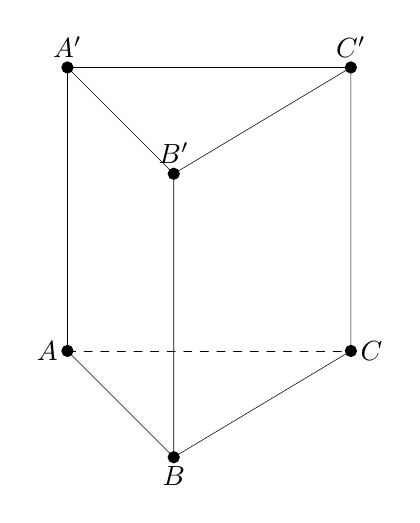
\begin{tikzpicture}[scale=0.9,>=stealth, font=\footnotesize, line join=round, line cap=round]
	\tkzDefPoints{0/0/A, 1.5/-1.5/B, 4/0/C}
	\coordinate (A') at ($(A)+(0,4)$);
	\coordinate (B') at ($(B)+(0,4)$);
	\coordinate (C') at ($(C)+(0,4)$);
	\tkzDrawPolygon(A',B',C')
	\tkzDrawSegments(A,A' B,B' C,C' A,B B,C)
	\tkzDrawSegments[dashed](A,C)
	\tkzDrawPoints[fill=black,size=4](A,B,C,A',B',C')
	\tkzLabelPoints[above](A',B',C')
	\tkzLabelPoints[below](B)
	\tkzLabelPoints[left](A)
	\tkzLabelPoints[right](C)
\end{tikzpicture}
\end{minipage}\hfill
\begin{minipage}[c]{0.52\textwidth}
\begin{tcolorbox}[codebox]
\begin{verbatim}
\begin{tikzpicture}[scale=0.9,>=stealth,...]
  \tkzDefPoints{0/0/A, 1.5/-1.5/B, 4/0/C}
  \coordinate (A') at ($(A)+(0,4)$);
  \coordinate (B') at ($(B)+(0,4)$);
  \coordinate (C') at ($(C)+(0,4)$);
  \tkzDrawPolygon(A',B',C')
  \tkzDrawSegments(A,A' B,B' C,C' A,B B,C)
  \tkzDrawSegments[dashed](A,C)
  \tkzDrawPoints[fill=black,size=4](A,B,C,A',B',C')
  \tkzLabelPoints[above](A',B',C')
\end{tikzpicture}
\end{verbatim}
\end{tcolorbox}
\end{minipage}

\vspace{0.5cm}

\subsection*{C.2. Hình hộp chữ nhật}
\noindent
\begin{minipage}[c]{0.45\textwidth}
\centering
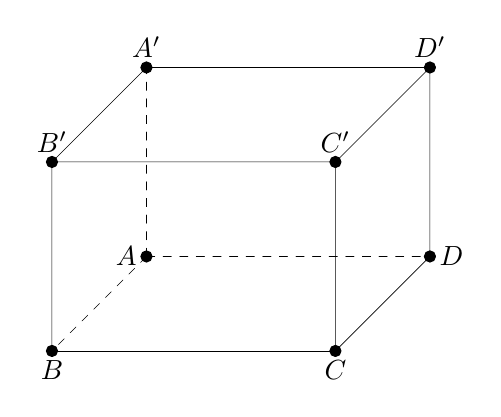
\begin{tikzpicture}[scale=0.8,>=stealth, font=\footnotesize, line join=round, line cap=round]
	\tkzDefPoints{0/0/A, -1.5/-1.5/B, 3/-1.5/C}
	\coordinate (D) at ($(A)+(C)-(B)$);
	\coordinate (A') at ($(A)+(0,3)$);
	\coordinate (B') at ($(B)+(0,3)$);
	\coordinate (C') at ($(C)+(0,3)$);
	\coordinate (D') at ($(D)+(0,3)$);
	\tkzDrawPolygon(A',B',C',D')
	\tkzDrawSegments(B,C C,D B,B' C,C' D,D')
	\tkzDrawSegments[dashed](A,B A,D A,A')
	\tkzDrawPoints[fill=black,size=4](A,B,C,D,A',B',C',D')
	\tkzLabelPoints[above](A',B',C',D')
	\tkzLabelPoints[below](B,C)
	\tkzLabelPoints[left](A)
	\tkzLabelPoints[right](D)
\end{tikzpicture}
\end{minipage}\hfill
\begin{minipage}[c]{0.52\textwidth}
\begin{tcolorbox}[codebox]
\begin{verbatim}
\begin{tikzpicture}[scale=0.8,>=stealth,...]
  \tkzDefPoints{0/0/A, -1.5/-1.5/B, 3/-1.5/C}
  \coordinate (D) at ($(A)+(C)-(B)$);
  \coordinate (A') at ($(A)+(0,3)$); 
  ... Tương tự tịnh tiến B', C', D'
  \tkzDrawPolygon(A',B',C',D')
  \tkzDrawSegments(B,C C,D B,B' C,C' D,D')
  \tkzDrawSegments[dashed](A,B A,D A,A')
  \tkzDrawPoints[fill=black,size=4](A,B,C...
\end{tikzpicture}
\end{verbatim}
\end{tcolorbox}
\end{minipage}

\vspace{1cm}

% -------------------------------------------------------------------------

\vspace{0.5cm}

\subsection*{C.3. Lăng trụ xiên tam giác}
\noindent
\begin{minipage}[c]{0.45\textwidth}
\centering
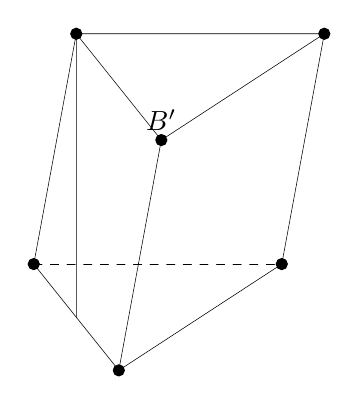
\begin{tikzpicture}[scale=0.9,>=stealth, font=\footnotesize, line join=round, line cap=round]
        \tkzDefPoints{0/0/A,1.2/-1.5/B,3.5/0/C}
        \coordinate (H) at ($(A)!1/2!(B)$);
        \coordinate (A') at ($(H)+(0,4)$);
        \tkzDefPointsBy[translation = from A to A'](B,C){B'}{C'}
        \tkzDrawPolygon(A,B,C,C',B',A')
        \tkzDrawSegments(A',C' B',B A',H)
        \tkzDrawSegments[dashed](A,C)
        \tkzDrawPoints[fill=black,size=4](A,C,B,A',B',C')
        \tkzLabelPoints[above](B')
\end{tikzpicture}
\end{minipage}\hfill
\begin{minipage}[c]{0.52\textwidth}
\begin{tcolorbox}[codebox]
\begin{verbatim}
\begin{tikzpicture}[scale=0.9,>=stealth,...]
  \tkzDefPoints{0/0/A,1.2/-1.5/B,3.5/0/C}
  \coordinate (H) at ($(A)!1/2!(B)$);
  \coordinate (A') at ($(H)+(0,4)$);
  \tkzDefPointsBy[translation = from A to A'](B,C){B'}{C'}
  \tkzDrawPolygon(A,B,C,C',B',A')
  \tkzDrawSegments(A',C' B',B A',H)
  \tkzDrawSegments[dashed](A,C)
\end{tikzpicture}
\end{verbatim}
\end{tcolorbox}
\end{minipage}


% -------------------------------------------------------------------------
\section*{D. NHÓM KHỐI TRÒN XOAY SERIES}
% -------------------------------------------------------------------------

\subsection*{D.1. Hình Nón}
\noindent
\begin{minipage}[c]{0.45\textwidth}
\centering
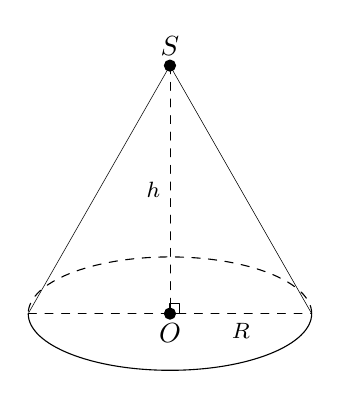
\begin{tikzpicture}[scale=0.9,>=stealth, font=\footnotesize, line join=round, line cap=round]
	\def \x{2} \def \y{0.8} \def \h{3.5}
	\coordinate (O) at (0,0);
	\coordinate (S) at ($(O)+(0,\h)$);
	\coordinate (l) at (180:\x cm and \y cm);
	\coordinate (r) at (0:\x cm and \y cm);
	\draw[dashed] (r) arc (0:180:\x cm and \y cm);
	\draw (r) arc (0:-180:\x cm and \y cm);
	\tkzDrawSegments(S,l S,r)
	\tkzDrawSegments[dashed](S,O l,r)
	\tkzDrawPoints[fill=black,size=4](O,S)
	\tkzLabelPoints[above](S);
	\tkzLabelPoints[below](O);
	\tkzMarkRightAngles[size=0.14](S,O,r)
	\node[below] at ($(O)!0.5!(r)$) {$R$};
	\node[left] at ($(O)!0.5!(S)$) {$h$};
\end{tikzpicture}
\end{minipage}\hfill
\begin{minipage}[c]{0.52\textwidth}
\begin{tcolorbox}[codebox]
\begin{verbatim}
\begin{tikzpicture}[scale=0.9,>=stealth,...]
  \def \x{2} \def \y{0.8} \def \h{3.5}
  \coordinate (O) at (0,0);
  \coordinate (S) at ($(O)+(0,\h)$);
  \coordinate (l) at (180:\x cm and \y cm);
  \coordinate (r) at (0:\x cm and \y cm);
  \draw[dashed] (r) arc (0:180:\x cm and \y cm);
  \draw (r) arc (0:-180:\x cm and \y cm);
  \tkzDrawSegments(S,l S,r)
  \tkzDrawSegments[dashed](S,O l,r)
\end{tikzpicture}
\end{verbatim}
\end{tcolorbox}
\end{minipage}

\vspace{0.5cm}

\subsection*{D.2. Hình Trụ}
\noindent
\begin{minipage}[c]{0.45\textwidth}
\centering
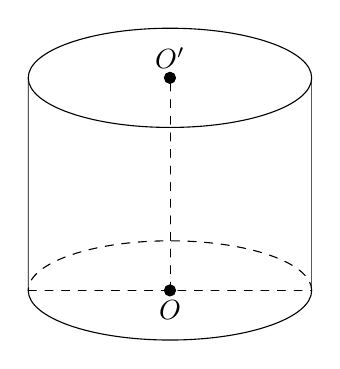
\begin{tikzpicture}[scale=0.9,>=stealth, font=\footnotesize, line join=round, line cap=round]
	\def \x{2} \def \y{0.7} \def \h{3}
	\coordinate (O) at (0,0);
	\coordinate (O') at ($(O)+(0,\h)$);
	\coordinate (Al) at (180:\x cm and \y cm);
	\coordinate (Ar) at (0:\x cm and \y cm);
	\coordinate (A'l) at ($(Al)+(0,\h)$);
	\coordinate (A'r) at ($(Ar)+(0,\h)$);
	
	\draw[dashed] (Ar) arc (0:180:\x cm and \y cm);
	\draw (Ar) arc (0:-180:\x cm and \y cm);
	\draw (A'r) arc (0:360:\x cm and \y cm);
	
	\tkzDrawSegments(Al,A'l Ar,A'r)
	\tkzDrawSegments[dashed](O,O' Al,Ar)
	\tkzDrawPoints[fill=black,size=4](O,O')
	\tkzLabelPoints[above](O');
	\tkzLabelPoints[below](O);
\end{tikzpicture}
\end{minipage}\hfill
\begin{minipage}[c]{0.52\textwidth}
\begin{tcolorbox}[codebox]
\begin{verbatim}
\begin{tikzpicture}[scale=0.9,>=stealth,...]
  \def \x{2} \def \y{0.7} \def \h{3}
  \coordinate (O) at (0,0);
  \coordinate (O') at ($(O)+(0,\h)$);
  \coordinate (Al) at (180:\x cm and \y cm); ...
  
  \draw[dashed] (Ar) arc (0:180:\x cm and \y cm);
  \draw (Ar) arc (0:-180:\x cm and \y cm);
  \draw (A'r) arc (0:360:\x cm and \y cm);
  
  \tkzDrawSegments(Al,A'l Ar,A'r)
  \tkzDrawSegments[dashed](O,O' Al,Ar)
\end{tikzpicture}
\end{verbatim}
\end{tcolorbox}
\end{minipage}

\vspace{0.5cm}

\subsection*{D.3. Hình Cầu}
\noindent
\begin{minipage}[c]{0.45\textwidth}
\centering
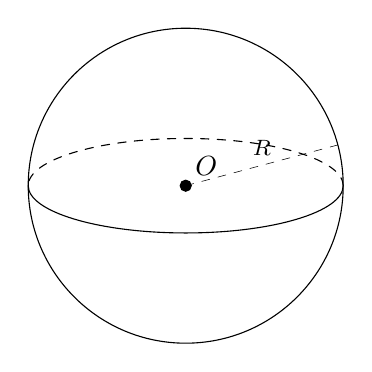
\begin{tikzpicture}[scale=1,>=stealth, font=\footnotesize, line join=round, line cap=round]
	\coordinate (O) at (0,0);
	\def\R{2}
	\draw (O) circle (\R);
	\draw[dashed] (\R,0) arc (0:180:\R cm and 0.3*\R cm);
	\draw (\R,0) arc (0:-180:\R cm and 0.3*\R cm);
	\tkzDrawPoints[fill=black,size=4](O)
	\tkzLabelPoints[above right](O)
	\coordinate (A) at (15:\R);
	\tkzDrawSegments[dashed](O,A)
	\node[above] at ($(O)!0.5!(A)$) {$R$};
\end{tikzpicture}
\end{minipage}\hfill
\begin{minipage}[c]{0.52\textwidth}
\begin{tcolorbox}[codebox]
\begin{verbatim}
\begin{tikzpicture}[scale=1,>=stealth,...]
  \coordinate (O) at (0,0);
  \def\R{2}
  \draw (O) circle (\R);
  \draw[dashed] (\R,0) arc 
         (0:180:\R cm and 0.3*\R cm);
  \draw (\R,0) arc 
         (0:-180:\R cm and 0.3*\R cm);
  \tkzDrawPoints[fill=black,size=4](O)
  \tkzLabelPoints[above right](O)
  \coordinate (A) at (15:\R);
  \tkzDrawSegments[dashed](O,A)
\end{tikzpicture}
\end{verbatim}
\end{tcolorbox}
\end{minipage}

\vspace{1cm}

% -------------------------------------------------------------------------
\section*{E. NHÓM VỊ TRÍ TƯƠNG ĐỐI (MẶT CẦU \& MẶT PHẲNG)}
% -------------------------------------------------------------------------

\subsection*{E.1. Mặt cầu tiếp xúc Mặt phẳng}
\noindent
\begin{minipage}[c]{0.45\textwidth}
\centering
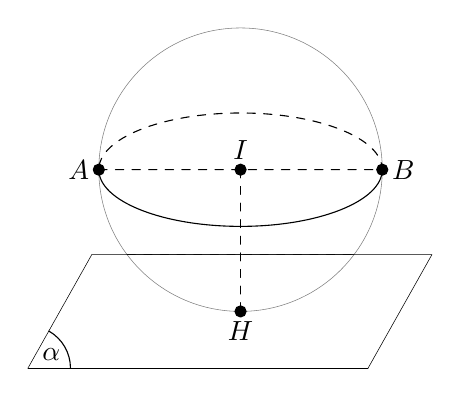
\begin{tikzpicture}[scale=0.9,>=stealth, font=\footnotesize, line join=round, line cap=round]
	\def \x{2} %bán kính trục lớn elip
	\def \y{0.8} %bán kính trục bé elip
	\coordinate (I) at (0,0);
	\coordinate (B) at (\x,0);
	\coordinate (A) at (-\x,0);
	\coordinate (H) at (-90:\x);
	\coordinate (m) at ($(H)+(-\x-1,-\y)$);
	\coordinate (n) at ($(H)+(\x-0.2,-\y)$);
	\coordinate (p) at ($(H)+(\x+0.7,\y)$);
	\coordinate (q) at ($(m)+(p)-(n)$);
	\tkzDrawCircle[radius](I,A)
	\draw[dashed] (A)--(B) arc (0:180:\x cm and \y cm);
	\draw (B) arc (0:-180:\x cm and \y cm);
	\tkzInterLC(p,q)(I,A)\tkzGetPoints{p'}{q'}
	\tkzDrawSegments[dashed](p',q' I,H)
	\tkzDrawSegments(q',q q,m m,n n,p p,p')
	\tkzDrawPoints[fill=black,size=4](A,B,I,H)
	\tkzLabelPoints[left](A)
	\tkzLabelPoints[right](B)
	\tkzLabelPoints[above](I)
	\tkzLabelPoints[below](H)
	\tkzMarkAngles[size=0.6cm,arc=l](n,m,q)
	\tkzLabelAngles[pos=0.38](n,m,q){$\alpha$}
\end{tikzpicture}
\end{minipage}\hfill
\begin{minipage}[c]{0.52\textwidth}
\begin{tcolorbox}[codebox]
\begin{verbatim}
\begin{tikzpicture}[scale=0.9,>=stealth,...]
  \def \x{2} \def \y{0.8} 
  \coordinate (I) at (0,0);
  \coordinate (B) at (\x,0);
  \coordinate (A) at (-\x,0);
  \coordinate (H) at (-90:\x);
  \coordinate (m) at ($(H)+(-\x-1,-\y)$); ...
  \tkzDrawCircle[radius](I,A)
  \draw[dashed] (A)--(B) arc (0:180:\x cm and \y cm);
  \draw (B) arc (0:-180:\x cm and \y cm);
  \tkzInterLC(p,q)(I,A)\tkzGetPoints{p'}{q'}
  \tkzDrawSegments[dashed](p',q' I,H)
  \tkzDrawSegments(q',q q,m m,n n,p p,p')
  \tkzMarkAngles[size=0.6cm,arc=l](n,m,q)
\end{tikzpicture}
\end{verbatim}
\end{tcolorbox}
\end{minipage}

\vspace{0.5cm}

\subsection*{E.2. Mặt cầu cắt Mặt phẳng}
\noindent
\begin{minipage}[c]{0.45\textwidth}
\centering
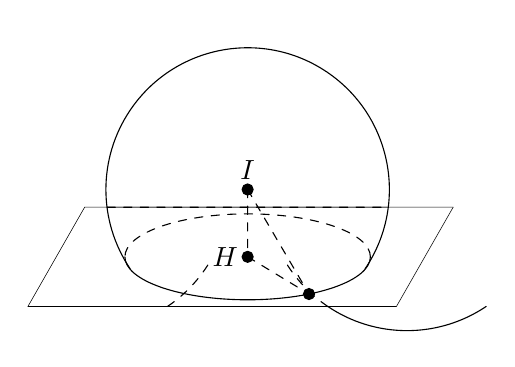
\begin{tikzpicture}[scale=0.9,>=stealth, font=\footnotesize, line join=round, line cap=round]
	\def \x{2} %bán kính trục lớn elip
	\def \y{0.7} %bán kính trục bé elip
	\coordinate (I) at (0,0);
	\coordinate (B) at (\x,0);
	\coordinate (A) at (-\x,0);
	\coordinate (H) at ($(0,-0.5*\x)+(0,0.05)$);
	\coordinate (M) at ($(H)+(-60:\x*0.866 cm and \y*0.866 cm)$);
	\coordinate (m) at ($(H)+(-\x-1.1,-\y)$);
	\coordinate (n) at ($(H)+(\x+0.1,-\y)$);
	\coordinate (p) at ($(H)+(\x+0.9,\y)$);
	\coordinate (q) at ($(m)+(p)-(n)$);
	\tkzInterLC(p,q)(I,A)\tkzGetPoints{p'}{q'}
	\tkzInterLC(m,n)(I,A)\tkzGetPoints{x}{y}
	\draw (-34:\x) arc (-34:214:\x);
	\draw (y) arc (-124:-56:\x);
	\draw (x)[dashed] arc (-56:-30:\x);
	\draw (y)[dashed] arc (-124:-150:\x);
	\draw[dashed] ($(-30:\x)+(0,0.05)$) arc (0:180:\x*0.866 cm and \y*0.866 cm);
	\draw ($(-30:\x)+(0,0.05)$) arc (0:-180:\x*0.866 cm and \y*0.866 cm);
	\draw[dashed] (p')--(q') (I)--(H) (I)--(M) (H)--(M);
	\tkzDrawSegments(q',q q,m m,n n,p p,p')
	\tkzDrawPoints[fill=black,size=4](I,H,M)
	\tkzLabelPoints[above](I)
	\tkzLabelPoints[left](H)
\end{tikzpicture}
\end{minipage}\hfill
\begin{minipage}[c]{0.52\textwidth}
\begin{tcolorbox}[codebox]
\begin{verbatim}
\begin{tikzpicture}[scale=0.9,>=stealth,...]
  \def \x{2} \def \y{0.7}
  \coordinate (I) at (0,0);
  \coordinate (B) at (\x,0); ...
  \tkzInterLC(p,q)(I,A)\tkzGetPoints{p'}{q'}
  \tkzInterLC(m,n)(I,A)\tkzGetPoints{x}{y}
  \draw (-34:\x) arc (-34:214:\x);
  \draw (y) arc (-124:-56:\x);
  \draw (x)[dashed] arc (-56:-30:\x);
  \draw (y)[dashed] arc (-124:-150:\x);
  \draw[dashed] ($(-30:\x)+(0,0.05)$) arc ...
  \draw ($(-30:\x)+(0,0.05)$) arc ...
  \draw[dashed] (p')--(q') (I)--(H)...
\end{tikzpicture}
\end{verbatim}
\end{tcolorbox}
\end{minipage}

\vspace{1cm}

% -------------------------------------------------------------------------
\section*{F. NHÓM ĐỒ THỊ HÀM SỐ \& HỆ TRỤC OXY}
% -------------------------------------------------------------------------

\subsection*{F.1. Đồ thị hàm Parabol (Bậc 2)}
\noindent
\begin{minipage}[c]{0.45\textwidth}
\centering
\begin{tikzpicture}[scale=0.8,>=stealth, font=\footnotesize, line join=round, line cap=round]
	\def\a{1} \def\b{-4} \def\c{3} % Hệ số
	\def\xmin{-1} \def\xmax{5}
	\def\ymin{-2} \def\ymax{4}

	\draw[<->] (\xmin,0)--(\xmax,0) node [below]{$x$};
	\draw[<->] (0,\ymin)--(0,\ymax) node [left]{$y$};
	\node at (0,0) [below left]{$O$};
	\clip (\xmin+0.1,\ymin+0.1) rectangle (\xmax-0.5,\ymax-0.1);
	\draw[smooth,samples=100, thick] plot(\x,{\a*(\x)^2+\b*(\x)+\c});
\end{tikzpicture}
\end{minipage}\hfill
\begin{minipage}[c]{0.52\textwidth}
\begin{tcolorbox}[codebox]
\begin{verbatim}
\begin{tikzpicture}[scale=0.8,>=stealth,...]
  \def\a{1} \def\b{-4} \def\c{3} 
  \def\xmin{-1} \def\xmax{5}
  \def\ymin{-2} \def\ymax{4}

  \draw[<->] (\xmin,0)--(\xmax,0) node [below]{$x$};
  \draw[<->] (0,\ymin)--(0,\ymax) node [left]{$y$};
  \node at (0,0) [below left]{$O$};
  \clip (\xmin+0.1,\ymin+0.1) rectangle ...
  \draw[smooth,samples=100, thick] 
    plot(\x,{\a*(\x)^2+\b*(\x)+\c});
\end{tikzpicture}
\end{verbatim}
\end{tcolorbox}
\end{minipage}

\vspace{0.5cm}

\subsection*{F.2. Đồ thị hàm số bậc 3}
\noindent
\begin{minipage}[c]{0.45\textwidth}
\centering
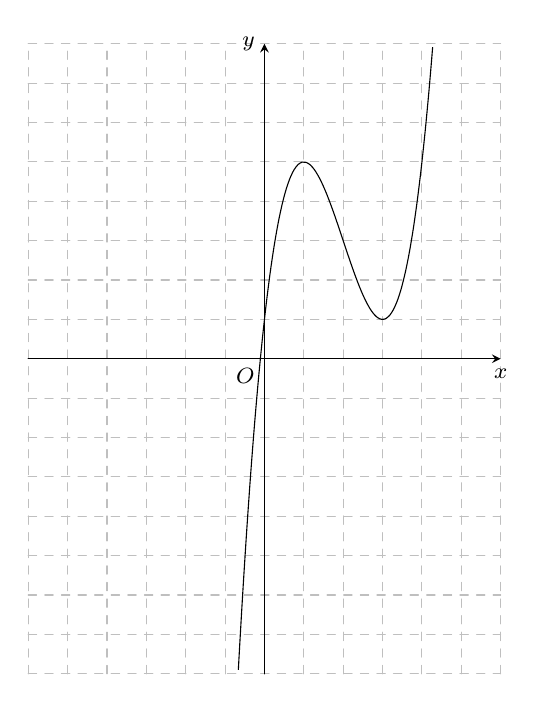
\begin{tikzpicture}[scale=0.5,>=stealth, font=\footnotesize, line join=round, line cap=round]
	\def\a{1} \def\b{-6} \def\c{9} \def\d{1} % Hệ số
	\def\xmin{-6} \def\xmax{6}
	\def\ymin{-8} \def\ymax{8} 
	\draw[color=gray!50,dashed] (\xmin,\ymin) grid (\xmax,\ymax); 
	\draw[->] (\xmin,0)--(\xmax,0) node [below]{$x$};
	\draw[->] (0,\ymin)--(0,\ymax) node [left]{$y$};
	\node at (0,0) [below left]{$O$};
	\clip (\xmin+0.1,\ymin+0.1) rectangle (\xmax-0.5,\ymax-0.1);
	\draw[smooth,samples=100] plot(\x,{\a*(\x)^3+\b*(\x)^2+\c*(\x)+\d});
\end{tikzpicture}
\end{minipage}\hfill
\begin{minipage}[c]{0.52\textwidth}
\begin{tcolorbox}[codebox]
\begin{verbatim}
\begin{tikzpicture}[scale=0.5,>=stealth,...]
  \def\a{1} \def\b{-6} \def\c{9} \def\d{1}
  \def\xmin{-6} \def\xmax{6}
  \def\ymin{-8} \def\ymax{8} 
  \draw[color=gray!50,dashed] (\xmin,\ymin) grid (\xmax,\ymax); 
  \draw[->] (\xmin,0)--(\xmax,0) node [below]{$x$};
  \draw[->] (0,\ymin)--(0,\ymax) node [left]{$y$};
  \node at (0,0) [below left]{$O$};
  \clip (\xmin+0.1,...);
  \draw[smooth,samples=100] plot(\x,{\a*(\x)^3+\b*(\x)^2+\c*(\x)+\d});
\end{tikzpicture}
\end{verbatim}
\end{tcolorbox}
\end{minipage}

\vspace{0.5cm}

\subsection*{F.3. Đồ thị hàm số trùng phương}
\noindent
\begin{minipage}[c]{0.45\textwidth}
\centering
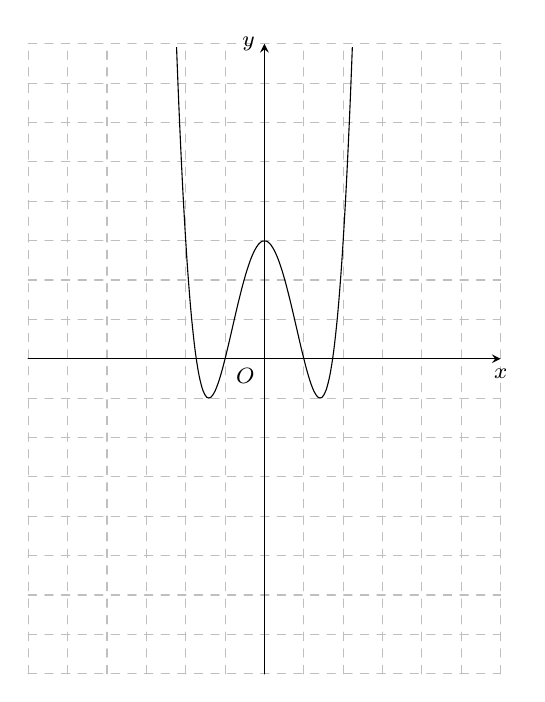
\begin{tikzpicture}[scale=0.5,>=stealth, font=\footnotesize, line join=round, line cap=round]
	\def\a{1} \def\b{-4} \def\c{3} % Hệ số
	\def\xmin{-6} \def\xmax{6}
	\def\ymin{-8} \def\ymax{8} 
	\draw[color=gray!50,dashed] (\xmin,\ymin) grid (\xmax,\ymax); 
	\draw[->] (\xmin,0)--(\xmax,0) node [below]{$x$};
	\draw[->] (0,\ymin)--(0,\ymax) node [left]{$y$};
	\node at (0,0) [below left]{$O$};
	\clip (\xmin+0.1,\ymin+0.1) rectangle (\xmax-0.5,\ymax-0.1);
	\draw[smooth,samples=100] plot(\x,{\a*(\x)^4+\b*(\x)^2+\c});
\end{tikzpicture}
\end{minipage}\hfill
\begin{minipage}[c]{0.52\textwidth}
\begin{tcolorbox}[codebox]
\begin{verbatim}
\begin{tikzpicture}[scale=0.5,>=stealth,...]
  \def\a{1} \def\b{-4} \def\c{3} 
  \def\xmin{-6} \def\xmax{6}
  \def\ymin{-8} \def\ymax{8} 
  \draw[color=gray!50,dashed] (\xmin,\ymin) grid (\xmax,\ymax); 
  \draw[->] (\xmin,0)--(\xmax,0) node [below]{$x$};
  \draw[->] (0,\ymin)--(0,\ymax) node [left]{$y$};
  \node at (0,0) [below left]{$O$};
  \clip (\xmin+0.1,...);
  \draw[smooth,samples=100] plot(\x,{\a*(\x)^4+\b*(\x)^2+\c});
\end{tikzpicture}
\end{verbatim}
\end{tcolorbox}
\end{minipage}

\vspace{0.5cm}

\subsection*{F.4. Đồ thị hàm số Nhất biến (Phân thức $\frac{ax+b}{cx+d}$)}
\noindent
\begin{minipage}[c]{0.45\textwidth}
\centering
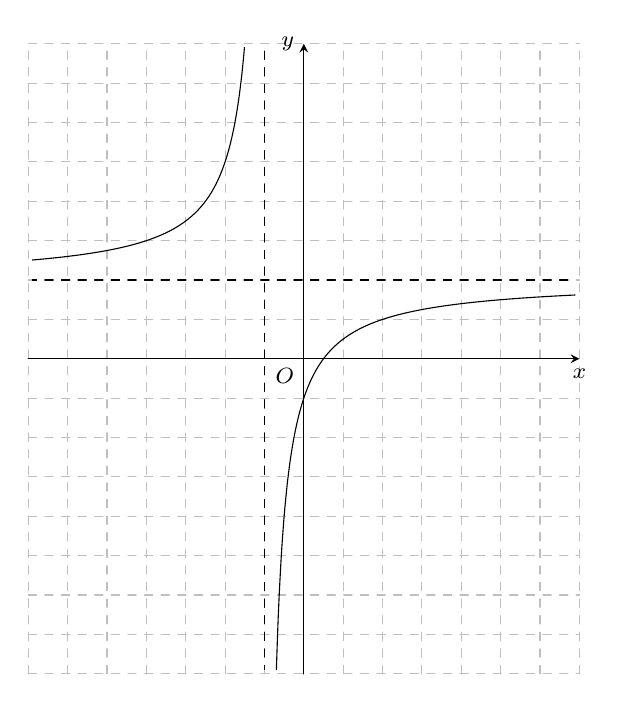
\begin{tikzpicture}[scale=0.5,>=stealth, font=\footnotesize, line join=round, line cap=round]
	\def\a{2} \def\b{-1} \def\c{1} \def\d{1} % Hệ số
	\def\xmin{-7} \def\xmax{7}
	\def\ymin{-8} \def\ymax{8}
	\draw[color=gray!50,dashed] (\xmin,\ymin) grid (\xmax,\ymax);
	\draw[->] (\xmin,0)--(\xmax,0) node [below]{$x$};
	\draw[->] (0,\ymin)--(0,\ymax) node [left]{$y$};
	\node at (0,0) [below left]{$O$};
	\clip (\xmin+0.1,\ymin+0.1) rectangle (\xmax-0.1,\ymax-0.1);
	\draw[smooth,samples=100,domain=\xmin:(-\d/\c-0.1)] plot(\x,{(\a*(\x)+\b)/(\c*(\x)+\d)});
	\draw[smooth,samples=100,domain=(-\d/\c+0.1:\xmax)] plot(\x,{(\a*(\x)+\b)/(\c*(\x)+\d)});
	\draw[dashed] (-\d/\c,\ymin)--(-\d/\c,\ymax);
	\draw[dashed] (\xmin,\a/\c)--(\xmax,\a/\c);
\end{tikzpicture}
\end{minipage}\hfill
\begin{minipage}[c]{0.52\textwidth}
\begin{tcolorbox}[codebox]
\begin{verbatim}
\begin{tikzpicture}[scale=0.5,>=stealth,...]
  \def\a{2} \def\b{-1} \def\c{1} \def\d{1}
  \def\xmin{-7} \def\xmax{7}
  \def\ymin{-8} \def\ymax{8}
  % Vẽ lưới và trục
  \clip (\xmin+0.1,\ymin+0.1) rectangle (\xmax-0.1,\ymax-0.1);
  % Vẽ miền x < -d/c
  \draw[smooth,domain=\xmin:(-\d/\c-0.1)] plot(\x,{(\a*(\x)+\b)/(\c*(\x)+\d)});
  % Vẽ miền x > -d/c
  \draw[smooth,domain=(-\d/\c+0.1:\xmax)] plot(\x,{(\a*(\x)+\b)/(\c*(\x)+\d)});
  % Tiệm cận đứng và ngang
  \draw[dashed] (-\d/\c,\ymin)--(-\d/\c,\ymax);
  \draw[dashed] (\xmin,\a/\c)--(\xmax,\a/\c);
\end{tikzpicture}
\end{verbatim}
\end{tcolorbox}
\end{minipage}

\vspace{0.5cm}

\subsection*{F.5. Đồ thị hàm lượng giác (Sin)}
\begin{center}
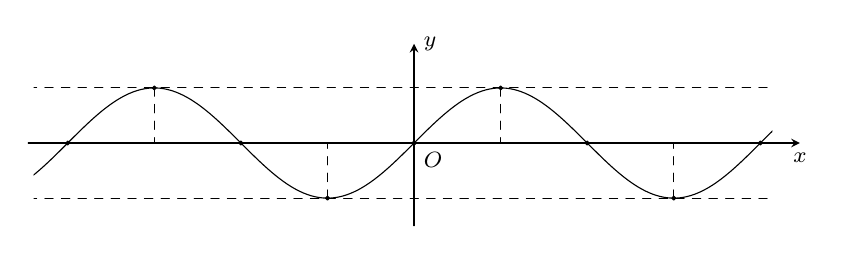
\begin{tikzpicture}[scale=0.7,>=stealth, font=\footnotesize, line join=round, line cap=round]
	\def\xmin{-7} \def\xmax{7} \def\ymin{-1.5} \def\ymax{1.8}
	\draw[->] (\xmin,0)--(\xmax,0) node [below]{$x$};
	\draw[->] (0,\ymin)--(0,\ymax) node [right]{$y$};
	\node at (0,0) [below right]{$O$};
	\clip (\xmin+0.1,\ymin+0.1) rectangle (\xmax-0.5,\ymax-0.1);
	\draw[smooth,samples=200,domain=\xmin:\xmax] plot(\x,{sin(\x r)});
	\draw[dashed] (\xmin,1)--(\xmax,1) (\xmin,-1)--(\xmax,-1);
	\foreach \x in {-2*pi,-1.5*pi,-pi,-0.5*pi,0}
	{\draw[fill=black] (\x,sin \x*180/pi) circle (1pt);
		\draw[dashed] (\x,sin \x*180/pi)--(\x,0);
		\draw[fill=black] (-\x,sin -\x*180/pi) circle (1pt);
		\draw[dashed] (-\x,sin -\x*180/pi)--(-\x,0);}
\end{tikzpicture}
\end{center}

\begin{tcolorbox}[codebox]
\begin{verbatim}
\begin{tikzpicture}[scale=0.7,>=stealth,...]
  \def\xmin{-7} \def\xmax{7} \def\ymin{-1.5} \def\ymax{1.8}
  \draw[->] (\xmin,0)--(\xmax,0) node [below]{$x$};
  \draw[->] (0,\ymin)--(0,\ymax) node [right]{$y$};
  \node at (0,0) [below right]{$O$};
  \clip (\xmin+0.1,\ymin+0.1) rectangle (\xmax-0.5,\ymax-0.1);
  \draw[smooth,samples=200,domain=\xmin:\xmax] plot(\x,{sin(\x r)});
  \draw[dashed] (\xmin,1)--(\xmax,1) (\xmin,-1)--(\xmax,-1);
  % Vẽ các điểm đặc biệt
  \foreach \x in {-2*pi,-1.5*pi,-pi,-0.5*pi,0}
  {\draw[fill=black] (\x,sin \x*180/pi) circle (1pt);
   \draw[dashed] (\x,sin \x*180/pi)--(\x,0);
   \draw[fill=black] (-\x,sin -\x*180/pi) circle (1pt);
   \draw[dashed] (-\x,sin -\x*180/pi)--(-\x,0);}
\end{tikzpicture}
\end{verbatim}
\end{tcolorbox}
\vspace{0.5cm}

\subsection*{F.6. Đồ thị hàm số Lũy thừa \& Logarit}
\noindent
\begin{minipage}[c]{0.45\textwidth}
\centering
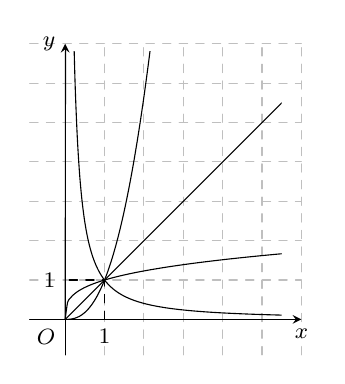
\begin{tikzpicture}[scale=0.5,>=stealth, font=\footnotesize, line join=round, line cap=round]
	\def\xmax{6} \def\ymax{7}
	\draw[color=gray!50,dashed] (-0.9,-0.9) grid (\xmax,\ymax);
	\draw[->] (-0.9,0)--(\xmax,0) node [below]{$x$};
	\draw[->] (0,-0.9)--(0,\ymax) node [left]{$y$};
	\node at (0,0) [below left]{$O$};
	\clip (-0.9,-0.9) rectangle (\xmax-0.5,\ymax-0.2);
	\draw[smooth,samples=100,domain=0:\xmax] plot(\x,{(\x)^2.5});
	\draw[smooth,samples=100,domain=0:\xmax] plot(\x,{\x});
	\draw[smooth,samples=100,domain=0:\xmax] plot(\x,{(\x)^0.3});
	\draw[smooth,samples=100,domain=0:\xmax] plot(\x,{(\x)^(-1.3)});
	\draw[dashed] (1,0) node[below]{$1$}--(1,1)--(0,1)node[left]{$1$};
\end{tikzpicture}
\end{minipage}\hfill
\begin{minipage}[c]{0.52\textwidth}
\begin{tcolorbox}[codebox]
\begin{verbatim}
\begin{tikzpicture}[scale=0.5,>=stealth,...]
  \def\xmax{6} \def\ymax{7}
  \draw[color=gray!50,dashed] (-0.9,-0.9) grid (\xmax,\ymax);
  \draw[->] (-0.9,0)--(\xmax,0) node [below]{$x$};
  \draw[->] (0,-0.9)--(0,\ymax) node [left]{$y$};
  \clip (-0.9,-0.9) rectangle (\xmax-0.5,\ymax-0.2);
  % Vẽ đường y = x^a theo các trường hợp a
  \draw[smooth,domain=0:\xmax] plot(\x,{(\x)^2.5});
  \draw[smooth,domain=0:\xmax] plot(\x,{\x});
  \draw[smooth,domain=0:\xmax] plot(\x,{(\x)^0.3});
  \draw[smooth,domain=0:\xmax] plot(\x,{(\x)^(-1.3)});
  \draw[dashed] (1,0) node[below]{$1$}--(1,1)--(0,1)node[left]{$1$};
\end{tikzpicture}
\end{verbatim}
\end{tcolorbox}
\end{minipage}

\vspace{1cm}

% -------------------------------------------------------------------------

\vspace{0.5cm}

\subsection*{F.7. Đồ thị hàm số Mũ ($a^x$)}
\noindent
\begin{minipage}[c]{0.45\textwidth}
\centering
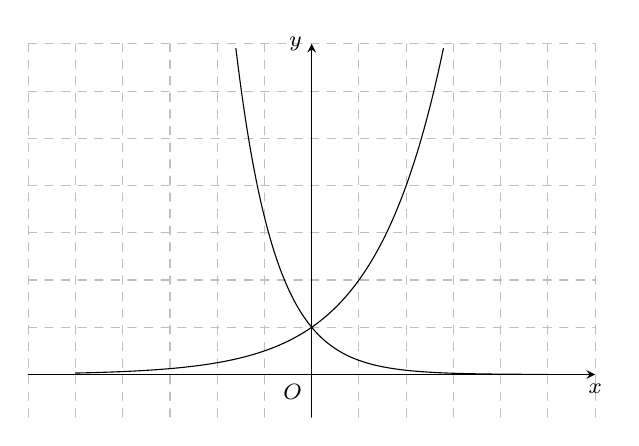
\begin{tikzpicture}[scale=0.6,>=stealth, font=\footnotesize, line join=round, line cap=round]
        \def\xmin{-6} \def\xmax{6} \def\ymax{7}
        \draw[color=gray!50,dashed] (\xmin,-0.9) grid (\xmax,\ymax);
        \draw[->] (\xmin,0)--(\xmax,0) node [below]{$x$};
        \draw[->] (0,-0.9)--(0,\ymax) node [left]{$y$};
        \node at (0,0) [below left]{$O$};
        \clip (\xmin,-0.9) rectangle (\xmax-0.1,\ymax-0.1);
        \draw[smooth,samples=100] plot(\x,{2^(\x)});
        \draw[smooth,samples=100] plot(\x,{0.3^(\x)});
\end{tikzpicture}
\end{minipage}\hfill
\begin{minipage}[c]{0.52\textwidth}
\begin{tcolorbox}[codebox]
\begin{verbatim}
\begin{tikzpicture}[scale=0.6,>=stealth,...]
  \def\xmin{-6} \def\xmax{6} \def\ymax{7}
  \draw[color=gray!50,dashed] (\xmin,-0.9) grid (\xmax,\ymax);
  \draw[->] (\xmin,0)--(\xmax,0) node [below]{$x$};
  \draw[->] (0,-0.9)--(0,\ymax) node [left]{$y$};
  \clip (\xmin,-0.9) rectangle (\xmax-0.1,\ymax-0.1);
  \draw[smooth,samples=100] plot(\x,{2^(\x)});
  \draw[smooth,samples=100] plot(\x,{0.3^(\x)});
\end{tikzpicture}
\end{verbatim}
\end{tcolorbox}
\end{minipage}

\vspace{0.5cm}

\subsection*{F.8. Đồ thị hàm số Logarit ($\log_a x$)}
\noindent
\begin{minipage}[c]{0.45\textwidth}
\centering
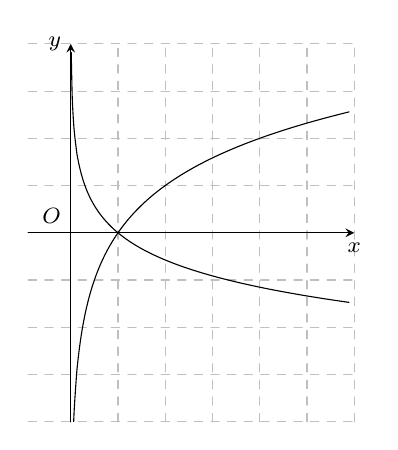
\begin{tikzpicture}[scale=0.6,>=stealth, font=\footnotesize, line join=round, line cap=round]
        \def\xmax{6} \def\ymin{-4} \def\ymax{4}
        \draw[color=gray!50,dashed] (-0.9,\ymin) grid (\xmax,\ymax);
        \draw[->] (-0.9,0)--(\xmax,0) node [below]{$x$};
        \draw[->] (0,\ymin)--(0,\ymax) node [left]{$y$};
        \node at (0,0) [above left]{$O$};
        \clip (-0.9,\ymin) rectangle (\xmax-0.1,\ymax-0.1);
        \draw[smooth,samples=300,domain=0.01:\xmax] plot(\x,{ln(\x)/ln(2)});
        \draw[smooth,samples=300,domain=0.01:\xmax] plot(\x,{ln(\x)/ln(0.3)});
\end{tikzpicture}
\end{minipage}\hfill
\begin{minipage}[c]{0.52\textwidth}
\begin{tcolorbox}[codebox]
\begin{verbatim}
\begin{tikzpicture}[scale=0.6,>=stealth,...]
  \def\xmax{6} \def\ymin{-4} \def\ymax{4}
  \draw[color=gray!50,dashed] (-0.9,\ymin) grid (\xmax,\ymax);
  \draw[->] (-0.9,0)--(\xmax,0) node [below]{$x$};
  \draw[->] (0,\ymin)--(0,\ymax) node [left]{$y$};
  \clip (-0.9,\ymin) rectangle (\xmax-0.1,\ymax-0.1);
  \draw[smooth,samples=300,domain=0.01:\xmax] plot(\x,{ln(\x)/ln(2)});
\end{tikzpicture}
\end{verbatim}
\end{tcolorbox}
\end{minipage}

\vspace{0.5cm}

\subsection*{F.9. Đồ thị hàm lượng giác (Cosin)}
\begin{center}
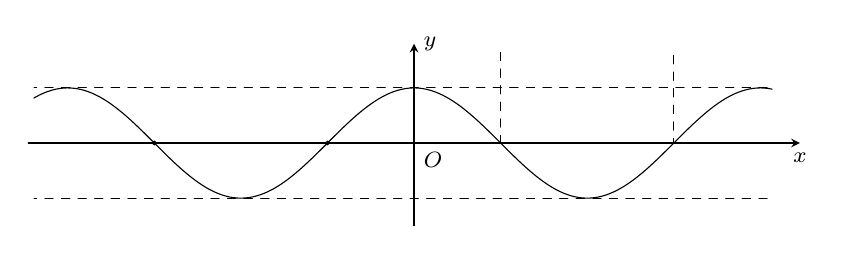
\begin{tikzpicture}[scale=0.7,>=stealth, font=\footnotesize, line join=round, line cap=round]
	\def\xmin{-7} \def\xmax{7} \def\ymin{-1.5} \def\ymax{1.8}
	\draw[->] (\xmin,0)--(\xmax,0) node [below]{$x$};
	\draw[->] (0,\ymin)--(0,\ymax) node [right]{$y$};
	\node at (0,0) [below right]{$O$};
	\clip (\xmin+0.1,\ymin+0.1) rectangle (\xmax-0.5,\ymax-0.1);
	\draw[smooth,samples=200,domain=\xmin:\xmax] plot(\x,{cos(\x r)});
	\draw[dashed] (\xmin,1)--(\xmax,1) (\xmin,-1)--(\xmax,-1);
	\foreach \x in {-1.5*pi,-0.5*pi,0.5*pi,1.5*pi}
	{\draw[fill=black] (\x,cos \x*180/pi) circle (1pt);
		\draw[dashed] (\x,cos \x*180/pi)--(\x,0);}
\end{tikzpicture}
\end{center}

\begin{tcolorbox}[codebox]
\begin{verbatim}
\begin{tikzpicture}[scale=0.7,>=stealth,...]
  \def\xmin{-7} \def\xmax{7} \def\ymin{-1.5} \def\ymax{1.8}
  \draw[->] (\xmin,0)--(\xmax,0) node [below]{$x$};
  \draw[->] (0,\ymin)--(0,\ymax) node [right]{$y$};
  \node at (0,0) [below right]{$O$};
  \clip (\xmin+0.1,\ymin+0.1) rectangle (\xmax-0.5,\ymax-0.1);
  \draw[smooth,samples=200,domain=\xmin:\xmax] plot(\x,{cos(\x r)});
  \draw[dashed] (\xmin,1)--(\xmax,1) (\xmin,-1)--(\xmax,-1);
  \foreach \x in {-1.5*pi,-0.5*pi,0.5*pi,1.5*pi}
  {\draw[fill=black] (\x,cos \x*180/pi) circle (1pt);
   \draw[dashed] (\x,cos \x*180/pi)--(\x,0);}
\end{tikzpicture}
\end{verbatim}
\end{tcolorbox}

\vspace{0.5cm}

\subsection*{F.10. Đồ thị hàm lượng giác (Tan)}
\begin{center}
\begin{tikzpicture}[scale=0.7,>=stealth, font=\footnotesize, line join=round, line cap=round]
	\def\xmin{-4.5} \def\xmax{4.5} \def\ymin{-3} \def\ymax{3}
	\draw[->] (\xmin,0)--(\xmax,0) node [below]{$x$};
	\draw[->] (0,\ymin)--(0,\ymax) node [right]{$y$};
	\node at (0,0) [below right]{$O$};
	\clip (\xmin+0.1,\ymin+0.1) rectangle (\xmax-0.5,\ymax-0.1);
	\draw[smooth,samples=200,domain=-1.4:1.4] plot(\x,{tan(\x r)});
	\draw[smooth,samples=200,domain=1.7:4.5] plot(\x,{tan(\x r)});
	\draw[smooth,samples=200,domain=-4.5:-1.7] plot(\x,{tan(\x r)});
	\foreach \x in {-1.5*pi,-0.5*pi,0.5*pi,1.5*pi}
	{\draw[dashed, color=red] (\x,\ymin)--(\x,\ymax);}
\end{tikzpicture}
\end{center}

\begin{tcolorbox}[codebox]
\begin{verbatim}
\begin{tikzpicture}[scale=0.7,>=stealth,...]
  \def\xmin{-4.5} \def\xmax{4.5} \def\ymin{-3} \def\ymax{3}
  \draw[->] (\xmin,0)--(\xmax,0) node [below]{$x$};
  \draw[->] (0,\ymin)--(0,\ymax) node [right]{$y$};
  \node at (0,0) [below right]{$O$};
  \clip (\xmin+0.1,\ymin+0.1) rectangle (\xmax-0.5,\ymax-0.1);
  \draw[smooth,samples=200,domain=-1.4:1.4] plot(\x,{tan(\x r)});
  \draw[smooth,samples=200,domain=1.7:4.5] plot(\x,{tan(\x r)});
  \draw[smooth,samples=200,domain=-4.5:-1.7] plot(\x,{tan(\x r)});
  \foreach \x in {-1.5*pi,-0.5*pi,0.5*pi,1.5*pi}
  {\draw[dashed, color=red] (\x,\ymin)--(\x,\ymax);}
\end{tikzpicture}
\end{verbatim}
\end{tcolorbox}

\vspace{0.5cm}

\subsection*{F.11. Đồ thị hàm lượng giác (Cotan)}
\begin{center}
\begin{tikzpicture}[scale=0.7,>=stealth, font=\footnotesize, line join=round, line cap=round]
	\def\xmin{-4.5} \def\xmax{4.5} \def\ymin{-3} \def\ymax{3}
	\draw[->] (\xmin,0)--(\xmax,0) node [below]{$x$};
	\draw[->] (0,\ymin)--(0,\ymax) node [right]{$y$};
	\node at (0,0) [below right]{$O$};
	\clip (\xmin+0.1,\ymin+0.1) rectangle (\xmax-0.5,\ymax-0.1);
	\draw[smooth,samples=200,domain=-3:-0.14] plot(\x,{cot(\x r)});
	\draw[smooth,samples=200,domain=0.14:3] plot(\x,{cot(\x r)});
	\draw[smooth,samples=200,domain=3.28:4.5] plot(\x,{cot(\x r)});
	\draw[smooth,samples=200,domain=-4.5:-3.28] plot(\x,{cot(\x r)});
	\foreach \x in {-1*pi,pi}
	{\draw[dashed, color=red] (\x,\ymin)--(\x,\ymax);}
\end{tikzpicture}
\end{center}

\begin{tcolorbox}[codebox]
\begin{verbatim}
\begin{tikzpicture}[scale=0.7,>=stealth,...]
  \def\xmin{-4.5} \def\xmax{4.5} \def\ymin{-3} \def\ymax{3}
  \draw[->] (\xmin,0)--(\xmax,0) node [below]{$x$};
  \draw[->] (0,\ymin)--(0,\ymax) node [right]{$y$};
  \node at (0,0) [below right]{$O$};
  \clip (\xmin+0.1,\ymin+0.1) rectangle (\xmax-0.5,\ymax-0.1);
  \draw[smooth,samples=200,domain=-3:-0.14] plot(\x,{cot(\x r)});
  \draw[smooth,samples=200,domain=0.14:3] plot(\x,{cot(\x r)});
  \draw[smooth,samples=200,domain=3.28:4.5] plot(\x,{cot(\x r)});
  \draw[smooth,samples=200,domain=-4.5:-3.28] plot(\x,{cot(\x r)});
  \foreach \x in {-1*pi,pi}
  {\draw[dashed, color=red] (\x,\ymin)--(\x,\ymax);}
\end{tikzpicture}
\end{verbatim}
\end{tcolorbox}


% -------------------------------------------------------------------------
\section*{G. NHÓM BẢNG BIẾN THIÊN \& BẢNG XÉT DẤU (TKZ-TAB)}
% -------------------------------------------------------------------------

\subsection*{G.1. Bảng biến thiên (Bậc 3 - 2 cực trị)}
\noindent
\begin{minipage}[c]{0.45\textwidth}
\centering
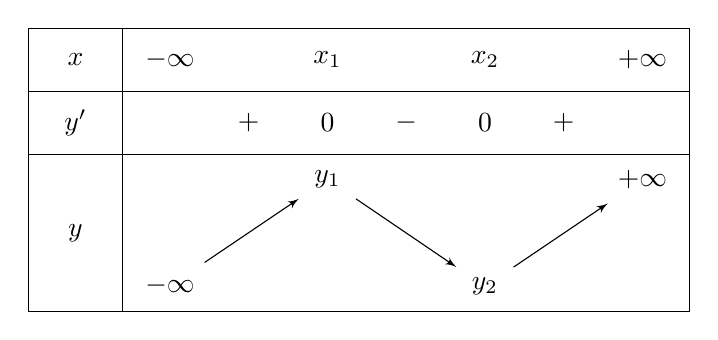
\begin{tikzpicture}[scale=1]
\tkzTabInit[nocadre=false,lgt=1.2,espcl=2,deltacl=0.6]
	{$x$ /0.8, $y'$ /0.8, $y$ /2}
	{$-\infty$,$x_1$,$x_2$,$+\infty$}
	\tkzTabLine{,+,$0$,-,$0$,+,}
	\tkzTabVar{-/$-\infty$,+/$y_1$,-/$y_2$,+/$+\infty$}
\end{tikzpicture}
\end{minipage}\hfill
\begin{minipage}[c]{0.52\textwidth}
\begin{tcolorbox}[codebox]
\begin{verbatim}
\begin{tikzpicture}[scale=1]
\tkzTabInit[nocadre=false,...] % Setup khung
  {$x$ /0.8, $y'$ /0.8, $y$ /2}
  {$-\infty$,$x_1$,$x_2$,$+\infty$}
  \tkzTabLine{,+,$0$,-,$0$,+,}
  \tkzTabVar{-/$-\infty$,+/$y_1$,-/$y_2$,+/$+\infty$}
\end{tikzpicture}
\end{verbatim}
\end{tcolorbox}
\end{minipage}

\vspace{0.5cm}

\subsection*{G.2. Bảng xét dấu 1 dòng}
\noindent
\begin{minipage}[c]{0.45\textwidth}
\centering
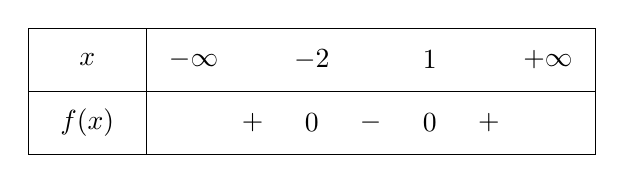
\begin{tikzpicture}[scale=1]
\tkzTabInit[nocadre=false,lgt=1.5,espcl=1.5,deltacl=0.6]
	{$x$ /0.8,$f(x)$ /0.8}
	{$-\infty$,$-2$,$1$,$+\infty$}
	\tkzTabLine{,+,$0$,-,$0$,+,}
\end{tikzpicture}
\end{minipage}\hfill
\begin{minipage}[c]{0.52\textwidth}
\begin{tcolorbox}[codebox]
\begin{verbatim}
\begin{tikzpicture}[scale=1]
\tkzTabInit[nocadre=false,lgt=1.5,espcl=1.5,...]
  {$x$ /0.8,$f(x)$ /0.8}
  {$-\infty$,$-2$,$1$,$+\infty$}
  \tkzTabLine{,+,$0$,-,$0$,+,}
\end{tikzpicture}
\end{verbatim}
\end{tcolorbox}
\end{minipage}

\vspace{0.5cm}

\subsection*{G.3. Bảng biến thiên (Bậc 3 - Vô nghiệm)}
\noindent
\begin{minipage}[c]{0.45\textwidth}
\centering
\begin{tikzpicture}[scale=1]
\tkzTabInit[nocadre=false,lgt=1.2,espcl=2,deltacl=0.6]
	{$x$/0.6,$y'$/0.6,$y$/2}
	{$-\infty$,$+\infty$}
	\tkzTabLine{,-,}
	\tkzTabVar{+/$+\infty$,-/$-\infty$}
\end{tikzpicture}
\end{minipage}\hfill
\begin{minipage}[c]{0.52\textwidth}
\begin{tcolorbox}[codebox]
\begin{verbatim}
\begin{tikzpicture}[scale=1]
\tkzTabInit[nocadre=false,...]
  {$x$/0.6,$y'$/0.6,$y$/2}
  {$-\infty$,$+\infty$}
  \tkzTabLine{,-,}
  \tkzTabVar{+/$+\infty$,-/$-\infty$}
\end{tikzpicture}
\end{verbatim}
\end{tcolorbox}
\end{minipage}

\vspace{0.5cm}

\subsection*{G.4. Bảng biến thiên (Hàm Nhất biến - Phân thức)}
\noindent
\begin{minipage}[c]{0.45\textwidth}
\centering
\begin{tikzpicture}[scale=1]
\tikzset{double style/.append style={double distance=1.5pt}}
\tkzTabInit[nocadre=false,lgt=1.2,espcl=2,deltacl=0.6]
	{$x$ /0.8,$y'$ /0.8,$y$ /2}
	{$-\infty$,$x_0$,$+\infty$}
	\tkzTabLine{,+,d,+,}
	\tkzTabVar{-/$y_0$,+D-/$+\infty$/$-\infty$,+/$y_0$}
\end{tikzpicture}
\end{minipage}\hfill
\begin{minipage}[c]{0.52\textwidth}
\begin{tcolorbox}[codebox]
\begin{verbatim}
\begin{tikzpicture}[scale=1]
\tikzset{double style/.append style={
   double distance=1.5pt}}
\tkzTabInit[nocadre=false,...]
  {$x$ /0.8,$y'$ /0.8,$y$ /2}
  {$-\infty$,$x_0$,$+\infty$}
  % Dùng ký hiệu 'd' (double line)
  \tkzTabLine{,+,d,+,}
  \tkzTabVar{-/$y_0$,+D-/$+\infty$/$-\infty$,+/$y_0$}
\end{tikzpicture}
\end{verbatim}
\end{tcolorbox}
\end{minipage}

\vspace{0.5cm}

\subsection*{G.5. Bảng xét dấu 3 dòng}
\begin{center}
\begin{tikzpicture}[scale=0.9]
\tkzTabInit[nocadre=false,lgt=2.5,espcl=2,deltacl=0.5]
	{$x$ /0.6,$x^2-x+6$ /0.6,$x-1$ /0.6,$\frac{x^2-x-6}{x-1}$ /1.1}
	{$-\infty$,$-2$,$1$,$3$,$+\infty$}
	\tkzTabLine{,+,$0$,-,|,-,$0$,+,}
	\tkzTabLine{,-,|,-,$0$,+,|,+,}
	\tkzTabLine{,-,$0$,+,||,-,$0$,+,}
\end{tikzpicture}
\end{center}

\begin{tcolorbox}[codebox]
\begin{verbatim}
\begin{tikzpicture}[scale=0.9]
\tkzTabInit[nocadre=false,lgt=2.5,...]
  {$x$, $x^2-x+6$, $x-1$, $\frac{...}{...}$}
  {$-\infty$,$-2$,$1$,$3$,$+\infty$}
  \tkzTabLine{,+,$0$,-,|,-,$0$,+,}
  \tkzTabLine{,-,|,-,$0$,+,|,+,}
  % Dùng ký tự || cho không xác định
  \tkzTabLine{,-,$0$,+,||,-,$0$,+,}
\end{tikzpicture}
\end{verbatim}
\end{tcolorbox}
\Closesolutionfile{ans}
\end{document}
